
\documentclass[10pt, letterpaper]{article}

% Packages
\usepackage[
    ignoreheadfoot,
    top=1.5cm,
    bottom=1.5cm,
    left=1.5cm,
    right=1.5cm,
    footskip=0.8cm
]{geometry}
\usepackage{datetime}
\newdateformat{monthyear}{\THEYEAR.\twodigit{\THEMONTH}}
\usepackage[explicit]{titlesec}
\usepackage{tabularx}
\usepackage{array}
\usepackage[dvipsnames]{xcolor}
\definecolor{primaryColor}{RGB}{0, 79, 144}
\definecolor{secondaryColor}{RGB}{100, 100, 100}
\usepackage{enumitem}
\usepackage{fontawesome5}
\usepackage{amsmath}
\usepackage[
    pdftitle={Yu Feng's CV},
    pdfauthor={Yu Feng},
    pdfcreator={LaTeX with RenderCV},
    colorlinks=true,
    urlcolor=primaryColor
]{hyperref}
\usepackage{eso-pic}
\usepackage{calc}
\usepackage{bookmark}
\usepackage{lastpage}
\usepackage{changepage}
\usepackage{paracol}
\usepackage{ifthen}
\usepackage{needspace}
\usepackage{iftex}
\usepackage{graphicx}
\usepackage{parskip}
\usepackage{tcolorbox}
\tcbuselibrary{skins}

% ATS compatibility
\ifPDFTeX
    \input{glyphtounicode}
    \pdfgentounicode=1
    \usepackage[T1]{fontenc}
    \usepackage[utf8]{inputenc}
    \usepackage{lmodern}
\fi

\usepackage[default, type1]{sourcesanspro}

% Settings
\AtBeginEnvironment{adjustwidth}{\partopsep0pt}
\pagestyle{empty}
\setcounter{secnumdepth}{0}
\setlength{\parindent}{0pt}
\setlength{\topskip}{0pt}
\setlength{\columnsep}{0.2cm}
\makeatletter
\let\ps@customFooterStyle\ps@plain
\patchcmd{\ps@customFooterStyle}{\thepage}{
    \color{secondaryColor}\small Yu Feng \textbar{}  Page \thepage{} of \pageref*{LastPage}
}{}{}
\makeatother
\pagestyle{customFooterStyle}

% Section formatting
\titleformat{\section}{
    \needspace{4\baselineskip}
    \large\color{primaryColor}
}{}{}{\textbf{#1}\hspace{0.2cm}\titlerule[0.8pt]\hspace{-0.1cm}}[]
\titlespacing{\section}{-1pt}{0.4cm}{0.3cm}

% Custom environments
\newenvironment{highlights}{
    \begin{itemize}[
        topsep=0.1cm,
        parsep=0.1cm,
        partopsep=0pt,
        itemsep=0.05cm,
        leftmargin=0.5cm
    ]
}{\end{itemize}}

\newenvironment{highlightsforbulletentries}{
    \begin{itemize}[
        topsep=0.1cm,
        parsep=0.1cm,
        partopsep=0pt,
        itemsep=0.05cm,
        leftmargin=0.4cm
    ]
}{\end{itemize}}

\newenvironment{onecolentry}{
    \begin{adjustwidth}{0.2cm}{0.2cm}
}{\end{adjustwidth}}

\newenvironment{twocolentry}[2][]{
    \onecolentry
    \def\secondColumn{#2}
    \setcolumnwidth{\fill, 3.2cm}
    \begin{paracol}{2}
}{\switchcolumn \raggedleft \secondColumn \end{paracol} \endonecolentry}

\newenvironment{threecolentry}[3][]{
    \onecolentry
    \def\thirdColumn{#3}
    \setcolumnwidth{1cm, \fill, 3.2cm}
    \begin{paracol}{3}
    {\raggedright #2} \switchcolumn
}{\switchcolumn \raggedleft \thirdColumn \end{paracol} \endonecolentry}

% Last updated text
\newcommand{\placelastupdatedtext}{
    \AddToShipoutPictureFG*{
        \put(
            \LenToUnit{\paperwidth-2.5cm},
            \LenToUnit{\paperheight-0.8cm}
        ){\vtop{{\null}\makebox[0pt][c]{
            \small\color{secondaryColor}\textit{Last updated: \monthyear\today}
        }}}
    }
}

% Custom href with external link icon
\let\hrefWithoutArrow\href
\renewcommand{\href}[2]{\hrefWithoutArrow{#1}{\ifthenelse{\equal{#2}{}}{ }{#2 }\raisebox{.15ex}{\footnotesize \faExternalLink*}}}
% \usepackage{ragged2e}

\begin{document}
    % \placelastupdatedtext

    % Header
    \noindent
    \begin{minipage}[t]{\dimexpr\textwidth-3cm-0.5cm}
        \vspace{5pt}
        \raggedright
        \strut
        \fontsize{30pt}{30pt}\selectfont\textbf{Yu Feng}\par
        \vspace{0.15cm}
        \fontsize{14pt}{14pt}\selectfont Ph.D. Candidate\par
        \vspace{0.3cm}
        \small
        \mbox{\faMapMarker*\hspace*{0.13cm}Hamamatsu, Japan}\par
            \vspace{0.1cm}
        % \mbox{\faCalendar*\hspace*{0.13cm}1991.09.02}\par
        %     \vspace{0.1cm}
        \mbox{\faEnvelope[regular]\hspace*{0.13cm}\hrefWithoutArrow{mailto:feng.yu.16@shizuoka.ac.jp}{feng.yu.16@shizuoka.ac.jp}}\par
            \vspace{0.1cm}
        \mbox{\faPhone*\hspace*{0.13cm}\hrefWithoutArrow{tel:+81-80-2289-9988}{+81-80-2289-9988}}\par
            \vspace{0.1cm}
        \mbox{\faLinkedin\hspace*{0.13cm}\href{https://www.linkedin.com/in/yu-feng-work/}{linkedin.com/in/yu-feng-work}}\par
        % \mbox{\faGithub\hspace*{0.13cm}\href{https://github.com/yu-feng}{github.com/yu-feng}}\par
    \end{minipage}%
    \hfill
    \begin{minipage}[t]{3cm}
        \vspace{0pt}
        \raisebox{-0.2cm}{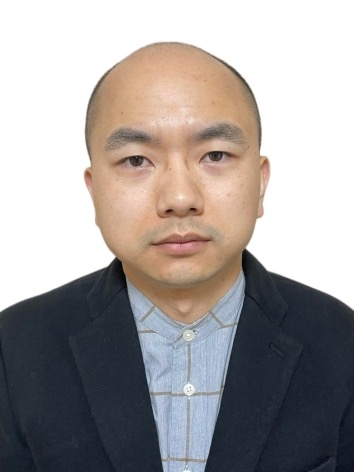
\includegraphics[width=3cm,keepaspectratio]{photo.jpg}}
    \end{minipage}

    % \vspace{0.2cm}
    % \noindent\rule{\textwidth}{0.4pt}

 \section{Motivation}
    % \begin{tcolorbox}[colback=gray!5, colframe=gray!5, boxrule=0pt, sharp corners, left=0.2cm, right=0.2cm]
        \begin{onecolentry}
        % \justifying
I am a Ph.D. candidate in Imaging Systems at Shizuoka University (expected graduation: September 2026), with 5+ years of experience in CMOS image sensor design and advanced imaging system development for biomedical and HDR applications. My research focuses on the development of a novel CMOS image sensor for multispectral skin tissue imaging, as well as the development of robust, motion- and ambient light–resistant imaging systems based on spatial frequency domain imaging (SFDI). I have also developed a single-frame HDR imaging system that effectively mitigates LED flicker and motion artifacts for automotive applications. I am the first author of two high-impact, peer-reviewed publications and have presented my work at multiple international and Japanese conferences. As a trilingual researcher (English, Japanese, Chinese), I thrive in global, interdisciplinary environments. I am currently seeking an R\&D role where I can contribute to the development of next-generation imaging technologies.

        \end{onecolentry}
    % \end{tcolorbox}

    \section{Education}
    \begin{threecolentry}{\textbf{Ph.D.}}{2023.10 – 2026.09 (Expected)}
        \textbf{Shizuoka University} \textbar{}  Hamamatsu, Japan \\ Nanovision Technology \\ Advisor: Prof. Kagawa Keiichiro \\ Research: Multi-tap CMOS Image Sensors for Biomedical Imaging
    \end{threecolentry}

    \begin{threecolentry}{\textbf{M.Eng.}}{2021.10 – 2023.09}
        \textbf{Shizuoka University} \textbar{}  Hamamatsu, Japan \\ Electronics Engineering \\
        Thesis: Performance Enhancement of SFDI with Multi-Tap Multi-Aperture CMOS Image Sensors
    \end{threecolentry}

    \begin{threecolentry}{\textbf{B.Eng.}}{2016.04 – 2020.03}
        \textbf{Shizuoka University} \textbar{}  Hamamatsu, Japan \\ Electronics Engineering
    \end{threecolentry}

    \section{Skills}
    \begin{onecolentry}
        \textbf{Programming Languages}: 
        % \begin{highlightsforbulletentries}
            % \item 
            MATLAB, C/C++,  Python, Verilog HDL
        % \end{highlightsforbulletentries}
    \end{onecolentry}
    % \vspace{0.1cm}
    \begin{onecolentry}
        \textbf{Hardware \& Tools}: CMOS Image Sensor architecture, VLSI Design (Cadence Virtuoso), FPGA (Quartus, ModelSim)
        % \end{highlightsforbulletentries}
    \end{onecolentry}
    % \vspace{0.1cm}
    \begin{onecolentry}
        \textbf{Languages}: English (Fluent, TOEIC 990/990, 2018), Japanese (Fluent, JLPT N1 passed, 2019), Chinese (Native)

    \end{onecolentry}



\section{Research Projects}
    \begin{twocolentry}{2024 – Present}
        \textbf{Ambient-Light-Robust 3-Wavelength Biomedical Imaging System}
        \begin{highlights}
            \item Developing a non-invasive quantitative skin measurement system robust to high ambient light environments (e.g. in hospital examination rooms) using pulsed illumination and an 8-tap CMOS image sensor, contributing to an anticipated >10x improvement in ambient light tolerance
        \end{highlights}
    \end{twocolentry}

    \begin{twocolentry}{2023 – 2024}
        \textbf{HDR Imaging System with LED Flicker and Motion Artifact Mitigation}
        \begin{highlights}
            \item Developed a programmable dynamic range  (56–110 dB) imaging system with LED flicker and motion artifact mitigation using a 4-tap  CMOS image sensor with the charge-splitting method for automotive and biomedical applications 
            \item Published in \textit{IEEE Sensors Journal} (2025.03)
        \end{highlights}
    \end{twocolentry}

    \begin{twocolentry}{2022 – 2023}
        \textbf{Motion-Artifact-Robust 3-Wavelength Biomedical Imaging System}
        \begin{highlights}
            \item Collaborated with University of California, Irvine to develop a non-invasive quantitative skin imaging system using an 8-tap CMOS image sensor designed to be robust against motion artifacts
            \item Designed hardware/software integration and conducted in vivo measurements
            \item Published in \textit{Journal of Biomedical Optics} (2024.01)
        \end{highlights}
    \end{twocolentry}

    \begin{twocolentry}{2021 – 2022}
        \textbf{Multi-Aperture Multi-Tap CMOS Image Sensor for Biomedical Imaging}
        \begin{highlights}
            \item Led VLSI design for a multi-aperture, multi-tap CMOS image sensor tailored for non-invasive multi-band biomedical imaging
            \item Fabricated in 2024, measurement in progress
        \end{highlights}
    \end{twocolentry}

    \section{Publications}
    \begin{twocolentry}{2025.03}
        1. \textbf{Programmable Dynamic Range HDR Imaging with LED-Flicker and Motion Artifact Mitigation Using a Four-Tap CMOS Image Sensor} \\
\underline{Yu Feng}, et al., \textit{IEEE Sensors Journal}, (2025). \href{https://doi.org/10.1109/JSEN.2025.3557801}{DOI: 10.1109/JSEN.2025.3557801}.
    \end{twocolentry}
  \vspace{0.1cm}
    \begin{twocolentry}{2024.01}
        2. \textbf{Motion-Resistant Three-Wavelength Spatial Frequency Domain Imaging System with Ambient Light Suppression Using an 8-Tap CMOS Image Sensor} \\
      \underline{Yu Feng}, et al., \textit{Journal of Biomedical Optics} 29.1 (2024): 016006. \href{https://doi.org/10.1117/1.JBO.29.1.016006}{DOI: 10.1117/1.JBO.29.1.016006}.
    \end{twocolentry}
  \vspace{0.1cm}
    \begin{twocolentry}{2025.03}
        3. \textbf{Spatial Frequency Domain Imaging System Using a Scanning Micro-Mirror} \\
        Kenta Nakazawa, \underline{Yu Feng}, et al., \textit{Sensors and Actuators A: Physical}, 387(2025): 116421. \\ \href{https://doi.org/10.1016/j.sna.2025.116421}{DOI: 10.1016/j.sna.2025.116421}.
    \end{twocolentry}
  \vspace{0.1cm}
    \begin{twocolentry}{2022.03}
        4. \textbf{Resolving Multi-Path Interference in Compressive Time-of-Flight Depth Imaging with a Multi-Tap Macro-Pixel Computational CMOS Image Sensor} \\
        Horio Masaya, \underline{Yu Feng}, et al., \textit{Sensors} 22.7 (2022): 2442. \href{https://doi.org/10.3390/s22072442}{DOI: 10.3390/s22072442}.
    \end{twocolentry}

    \section{Conference Presentations (Selected)}
    % (Presenting Author: \textbf{Yu Feng})
    \begin{twocolentry}{2025.06 (Expected)}
        1. \textbf{Room-Light Operation of a Three-Wavelength Spatial Frequency Domain Imaging System Using Pulsed Illumination and an 8-Tap CMOS Image Sensor} \\
        \underline{Yu Feng}, et al., \textit{European Conference on Biomedical Optics 2025}, Munich, Germany
    \end{twocolentry}
  \vspace{0.1cm}
    \begin{twocolentry}{2025.06}
        2. \textbf{Programmable Dynamic Range Extension up to 110 dB Based on Charge-Splitting Method with 4-Tap CMOS Image Sensor} \\
                \underline{Yu Feng}, et al., \textit{International Image Sensor Workshop 2025}, Hyogo, Japan
    \end{twocolentry}
  \vspace{0.1cm}
    \begin{twocolentry}{2024.07}
        3. \textbf{Multi-Tap CMOS Image Sensor with Programmable Functional Exposure: Application to Structured Light Based Quantitative Tissue Imaging} \\
                \underline{Yu Feng}, et al., \textit{Optica Imaging Congress 2024}, Toulouse, France
    \end{twocolentry}

    \section{Professional Experience}
    \begin{twocolentry}{2021.10 – Present}
        \textbf{Research and Teaching Assistant}, Shizuoka University \textbar{}   Hamamatsu, Japan
        \begin{highlights}
            \item Conducting R\&D on multi-tap CMOS image sensors for biomedical/HDR imaging, focusing on digital design and system integration
            \item Supporting undergraduate programming courses (Python and Verilog HDL), assisting with lectures, assignments, and student queries
        \end{highlights}
    \end{twocolentry}

    \begin{twocolentry}{2020.04 – 2021.09}
        \textbf{QA Engineer}, Meidensha \textbar{}   Nagoya, Japan
        \begin{highlights}
            \item Conducted quality assurance for electric vehicle motors
        \end{highlights}
    \end{twocolentry}


    \section{Awards \& Honors}
    \begin{onecolentry}
        \begin{highlightsforbulletentries}
            \item \textbf{Graduate School Scholarship}, Amano Foundation \hfill 2023.09 – 2026.09
            \item \textbf{Outstanding Academic Records}, Shizuoka University\hfill 2024.04 – 2025.09
        \end{highlightsforbulletentries}
    \end{onecolentry}

    % \section{Hobbies}
    % \begin{onecolentry}
    %     \begin{highlightsforbulletentries}
    %         \item Traveling, exploring diverse cultures
    %         \item Watching movies, particularly sci-fi and documentaries
    %     \end{highlightsforbulletentries}
    % \end{onecolentry}

\end{document}